\section{Executive recommendation}

\subsection{Recommended scientific thesis}

The research plan remains viable, but the central contribution should no longer be described as ``SAFE plus early triggering plus critic-guided flow.'' Recent work already studies calibrated VLA verification, recovery windows, counterfactual recovery labels, subtask backtracking, and critic- or reward-guided action generation~\cite{checkvla,b2ff,cyclevla,afil,rover,qvgm,guidedactionflow}. The stronger and more defensible thesis is:

\begin{quote}
\textbf{A failure detector's confidence is not its intervention value. Long-horizon VLA recovery has a state-, stage-, delay-, and operator-dependent deadline that must be measured causally and predicted directly.}
\end{quote}

The method should therefore learn whether intervention has positive value, when that value disappears, and which recovery action or operator should be selected. SAFE remains scientifically important as (i) the internal action-policy representation being adapted, (ii) a strong terminal-failure baseline, and (iii) a candidate input to the recovery-value model. It should not be assumed to be a value function.

\subsection{Primary paper endpoint}

The final primary endpoint is not detector ROC-AUC. It is the equal-task absolute improvement in final RoboCasa365 task success produced by the complete deployable system relative to the strongest frozen non-oracle baseline, under a matched intervention and inference budget. Detector ranking, warning time, stage recovery, and candidate-selection accuracy are mechanistic secondary endpoints that explain the task-success result.

\sciencenote{Recommended contribution statement.}{The paper introduces exact-prefix counterfactual recoverability curves, demonstrates that terminal-failure likelihood and causal intervention value diverge, and learns a stage-aware utility gate that decides whether, when, and how to recover while controlling harmful interventions.}

\subsection{Starting evidence}

Table~\ref{tab:starting-evidence} summarizes the evidence already available in the repository. The strongest current detector evidence is a frozen prospective Xiaomi shadow test, but it did not execute recovery. The five-task stage-aware development gain was tested on 250 new identity-disjoint parents and did not transfer. Phase~2 established exact complete-snapshot branching on a bounded two-task validation. Phase~3 found zero completion across 80 short-suffix candidates. Phase~3B then extended the same exact branches to 30 genuine replans for ArrangeTea and 16 for CuttingToolSelection. Its 140-branch engineering audit passed, but the full screen found only one mixed snapshot, 1.25 percentage points of oracle-over-random headroom, and no full-task successes. This is sufficient to reject local chunk reranking for the frozen two-task candidate set. The subsequent higher-level operator screen completed 160 scientific suffixes with all engineering gates passing, but continuation reached 22.5\% stage completion versus 17.5\% for every intervention. Oracle operator routing added zero completion gain and no operator passed. The active proposal is now one common-stage-entry timing diagnostic; candidate-critic training, operator-router training, and broad surface collection remain blocked.

\begingroup
\small
\begin{longtable}{P{0.22\textwidth}P{0.36\textwidth}P{0.32\textwidth}}
\caption{Current evidence and the strongest defensible interpretation. ``Prospective shadow'' means the detector bundle was frozen before scoring new trajectories, but the detector did not change policy execution.}
\label{tab:starting-evidence}\\
\toprule
Component & Evidence & Current interpretation \\
\midrule
\endfirsthead
\toprule
Component & Evidence & Current interpretation \\
\midrule
\endhead
Xiaomi matched-FPR shadow test & 760 balanced primary rollouts. Staged SAFE plus time reached TPR 0.668 at FPR 0.050, versus time-only TPR 0.632 at FPR 0.047. The timing gain was 0.0259 task horizons and its bootstrap interval crossed zero; only 2.9\% of failures were detected by the 25\% landmark. & Modest prospective classification gain; overall early-warning gate failed; no recovery claim. \\
Full-parent stage-aware confirmation & Development selection favored conditioned SAFE (ROC 0.696 versus 0.592 terminal). On 250 frozen, identity-disjoint parents, conditioned SAFE reached 0.489 versus 0.523 terminal, 0.563 SAFE38, and 0.500 time-only. All preregistered gates failed. & The development gain did not replicate. Predicate-stage-aware SAFE remains a baseline or model input, not a deployable trigger contribution. \\
State-context follow-up & A new 250-parent cohort recorded a 240-dimensional proprioceptive state history. Development selected stage SAFE at 0.693, context at 0.691, and terminal at 0.690. On the locked 85-parent retrospective holdout, stage reached 0.584, context 0.566, terminal 0.470, and time-only 0.500; both primary contrast intervals crossed zero. & Descriptive evidence of task-specific signal, not prospective confirmation. State context did not improve the selected ranking or the matched-FPR operating point. \\
RLDX Subtask-SAFE & Raw segment ROC 0.734 fell to parent-aware ROC 0.558, while an elapsed-time baseline reached 0.740. Frozen causal-prefix variants remained near chance. & Retrospective segment separation did not translate to online intervention evidence. \\
Recovery infrastructure & Ordered subtask anchors, environment reset, EEF recovery, continuation, and Xiaomi deterministic best-of-$K$ proposals exist. & Useful implementation base; existing runs do not establish randomized recovery utility. \\
Complete snapshot replay & On two tasks, 10 of 10 eligible parents produced 20 of 20 snapshots and 140 of 140 branches: 80 explicit candidates, 40 same-seed repeats, and 20 environment-only controls. There were zero branch errors, exact repeated requests/actions/observations/causal transitions, 100\% repeated-suffix agreement, and 100\% candidate diversity. & Phase~2 engineering validity passed and supplied the immutable states and branches used by Phases~3 and 3B. \\
Counterfactual opportunity pilot & The 10-parent, 20-snapshot Phase~3 analysis found zero stage completions and zero full-task successes among 80 candidates. Mixed-outcome fraction, random and oracle completion, oracle headroom, nominal completion, and lowest-SAFE completion were all zero. All candidates ended at the 64-step suffix after only four genuine replans. & The short-suffix proposal--horizon pair had no measurable ranking opportunity. It motivated one bounded training-horizon continuation rather than critic training. \\
Training-horizon continuation & Phase~3B passed all engineering gates on 10 parents, 20 snapshots, 140 branches, and 140 same-runtime prefix references with zero errors. Among 80 candidates, task-macro random stage completion was 0.2375, oracle-best-of-four was 0.2500, and nominal was 0.2000. Only one snapshot from one ArrangeTea parent was mixed; oracle-minus-random was 0.0125, oracle-minus-nominal was 0.0500, and full-task success was zero. & The local-candidate scientific gate failed. Candidate-critic and five-task candidate scaling are blocked. The subsequently completed operator screen is reported below. \\
Higher-level operator screen & 160 scientific suffixes on the same 10 parents and 20 snapshots; zero errors and every engineering gate passed. Continuation reached 22.5\% stage completion and 20.0\% endpoint retention; every intervention reached 17.5\% completion. No parent benefited on average, oracle routing gain was zero, and full-task success was zero. & Completed negative developmental screen. No useful fixed operator or router target; next test a bounded common-stage-entry timing protocol, not SAFE-triggered recovery. \\
\bottomrule
\end{longtable}
\endgroup

\begin{figure}[H]
\centering
\begin{subfigure}[t]{0.48\textwidth}
  \centering
  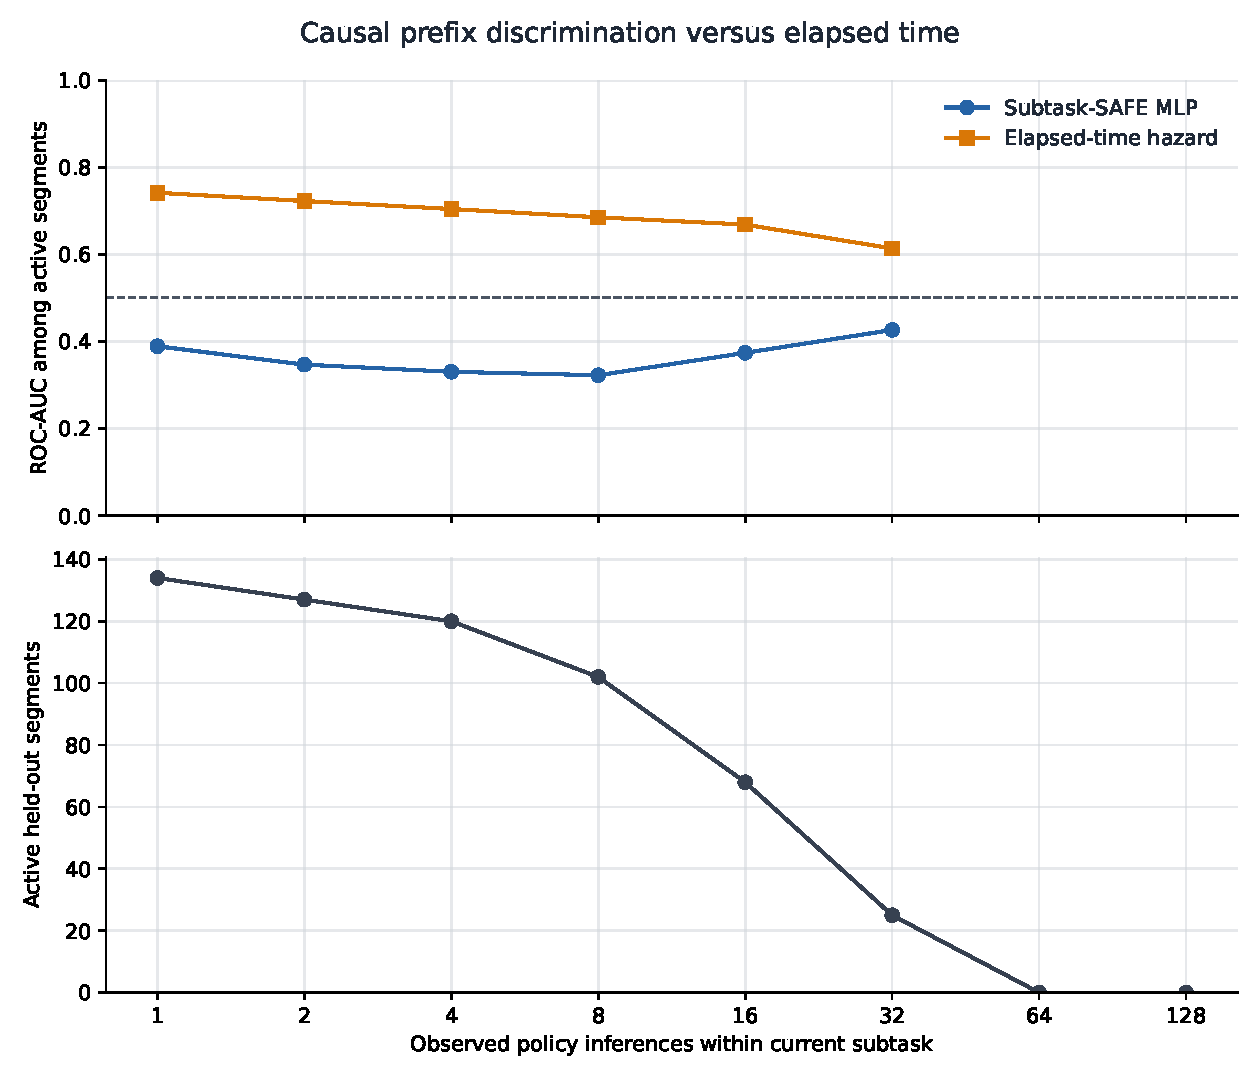
\includegraphics[width=\linewidth]{subtask_causal_prefix_roc.pdf}
  \caption{Causal prefix evaluation exposes the gap between retrospective Subtask-SAFE ranking and online utility.}
\end{subfigure}\hfill
\begin{subfigure}[t]{0.48\textwidth}
  \centering
  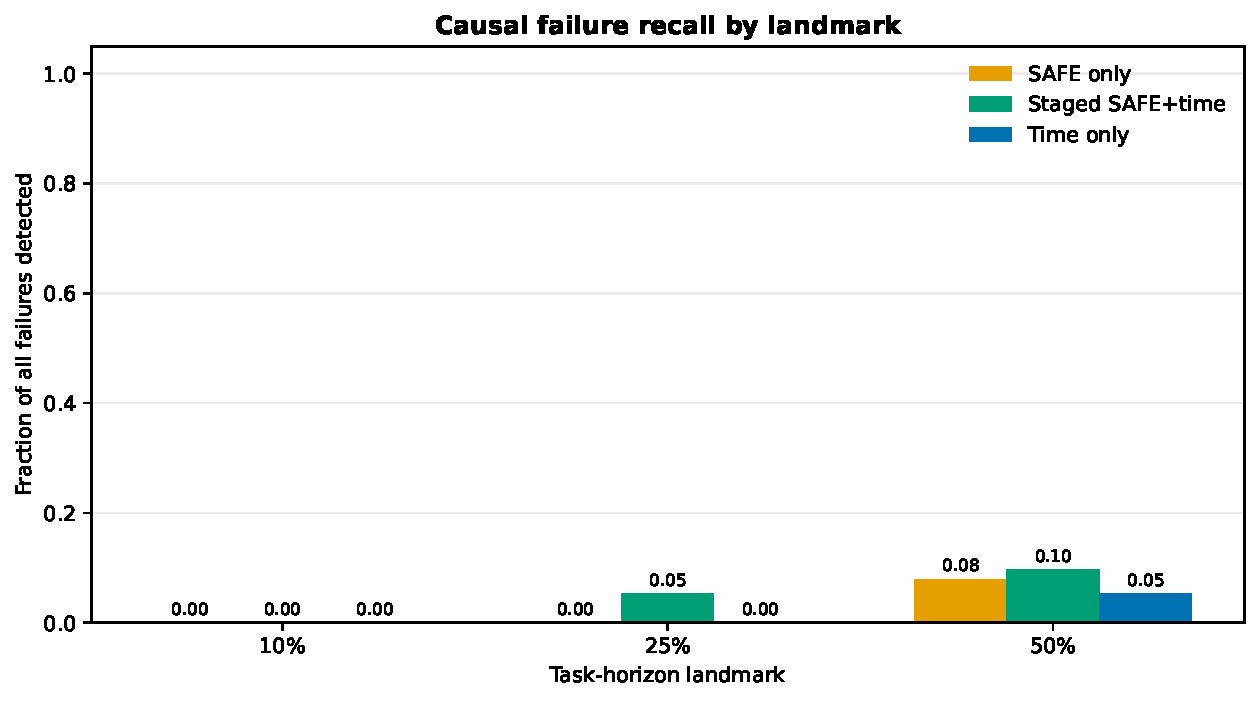
\includegraphics[width=\linewidth]{xr1_matched_fpr_recall_by_landmark.pdf}
  \caption{The frozen Xiaomi shadow test achieved low early-landmark recall on composite failures.}
\end{subfigure}
\caption{The research plan begins from negative causal and timing evidence rather than from retrospective ROC alone. Figures are reproduced from the checksum-backed full report.}
\label{fig:starting-point}
\end{figure}

\subsection{Dependency-gated roadmap}

\begin{longtable}{P{0.07\textwidth}P{0.28\textwidth}P{0.28\textwidth}P{0.269\textwidth}}
\caption{Experiment dependency structure. Each expensive phase is conditional on the preceding scientific or engineering gate.}\label{tab:roadmap}\\
\toprule
Phase & Experiment & Positive result & If the gate fails \\
\midrule
\endfirsthead
\toprule
Phase & Experiment & Positive result & If the gate fails \\
\midrule
\endhead
0 & Protocol freeze and evidence audit & Artifacts, identities, and endpoints are immutable and reproducible. & Repair integrity; do not collect. \\
1 & Frozen stage-aware confirmation \bad & Early stage-aware ranking transfers to new parents. & \textbf{Observed: gate failed.} SAFE becomes a baseline/input, not the trigger contribution. \\
2 & Complete snapshot replay \good & \textbf{Observed: gate passed.} Same state and randomness reproduced while declared candidate seeds created controlled alternatives. & Not applicable; preserve the passing bundle and hashes. \\
3 & Short-horizon opportunity screen \bad & \textbf{Observed: bounded gate failed.} Mixed-outcome fraction and oracle headroom were both zero across 80 candidates. & Preserve the negative result; do not train a critic or reinterpret generic progress as success. \\
3B & Training-horizon continuation \bad & \textbf{Observed: engineering passed, scientific gate failed.} Only $1/20$ snapshots was mixed; oracle-minus-random was 0.0125 and no candidate achieved full-task success. & Local chunk reranking is closed for this frozen set; do not train or scale a candidate critic. \\
3B-R & Higher-level operator screen \bad & \textbf{Observed: engineering passed, scientific gate failed.} Continuation was best; every intervention lost five completion points and oracle routing gain was zero. & Preserve the result; no router or fixed executor is supported at these states. \\
3B-T & Common-stage-entry timing diagnostic \planned & Earlier application yields useful paired operator advantage under a shared base and endpoint. & If useful value remains absent, redesign the executor or report a diagnostic benchmark. \\
4 & Recoverability surfaces & Intervention value varies meaningfully with delay, stage, and operator. & Narrow to a diagnostic benchmark or improve operators. \\
5 & Recovery-value critic & The learned critic predicts and ranks causal utility on sealed parents/tasks. & Do not guide the policy; preserve the benchmark result. \\
6 & Prospective best-of-$K$ selection & Critic selection beats random $K=4$ under identical candidates. & No flow guidance; critic is not actionably causal. \\
7 & Frozen end-to-end intervention & Final task success improves without excessive harm. & No deployable recovery-system claim. \\
8 & Differentiable flow guidance & Guided $K=1$ matches critic $K=4$ at lower cost and no safety loss. & Retain discrete critic reranking. \\
9 & Generalization and physical validation & Benefit survives held-out tasks/scenes and another policy or robot. & Scope the paper to same-policy RoboCasa365. \\
\bottomrule
\end{longtable}

\cautionnote{Planning thresholds.}{The numerical gates in this report are proposed research decisions, not official venue requirements. Final powered sample sizes must be frozen from blinded pilot variance and the exact hierarchical analysis.}

\sciencenote{Current decision.}{Preserve Phase~2 and the completed negative candidate and operator screens. The 160-suffix operator screen found no fixed-operator benefit and zero oracle routing headroom; training a router or scaling those arms is unsupported. Run at most one separately registered common-stage-entry timing diagnostic (Section~\ref{sec:next-timing-study}), followed by fresh-parent validation only if it identifies useful intervention value. SAFE-triggered recovery remains untested and deferred.}
